\documentclass[a4paper,12pt]{article}
\usepackage{graphicx} 
\usepackage{amsmath}
\usepackage{amssymb}
\usepackage{listings}
\usepackage{xcolor} 

\lstdefinestyle{mystyle}{
    language=C,
    basicstyle=\ttfamily\footnotesize,
    keywordstyle=\color{blue}\bfseries,
    commentstyle=\color{gray},
    stringstyle=\color{red},
    numberstyle=\tiny\color{gray},
    numbers=left,
    stepnumber=1,
    showstringspaces=false,
    breaklines=true,
    backgroundcolor=\color{lightgray!10},
    frame=single,
    rulecolor=\color{black},
}
\lstset{style=mystyle}

\title{Digital Clock using Arduino and 7-Segment Displays}
\author{Srihaas Gunda-EE24BTECH11026}
\date{}
\begin{document}

\maketitle

\tableofcontents  
\newpage  

\section{Introduction}
A digital clock is a very useful device used to display time in 24-hour format. This aim of the project is to make a digital clock using  Arduino.

\section{Components used}
The following components were used:
\begin{itemize}
    \item Arduino Uno
    \item Breadboard
    \item Six 7-segment displays
    \item A 7447 BCD to 7-segment decoders
    \item Push buttons for setting time
    \item Resistors($220 \Omega$) and wiring
    \item Power source
\end{itemize}

\section{Circuit Design}
The 7-segment displays are connected to each other and then one of them is connected to the pins of the 7447 according to  the table below

\begin{table}[h]
    \centering
    \begin{tabular}{|c|c|c|c|c|c|c|c|}
        \hline
        \textbf{7447} & $\bar{a}$ & $\bar{b}$ & $\bar{c}$ & $\bar{d}$ & $\bar{e}$ & $\bar{f}$ & $\bar{g}$ \\ \hline
        \textbf{Display} & a & b & c & d & e & f & g \\ \hline
    \end{tabular}
\end{table}
The remaining pins of 7447 which are to be connected to the arduino are as follows
\begin{table}[h]
    \centering
    \begin{tabular}{|c|c|c|c|c|}
        \hline
        \textbf{7447} & D & C & B & A \\ \hline
        \textbf{Arduino} & 5 & 4 & 3 & 2 \\ \hline
    \end{tabular}
\end{table}

\begin{figure}[h]
    \centering
    \begin{minipage}{0.48\textwidth}
        \centering
        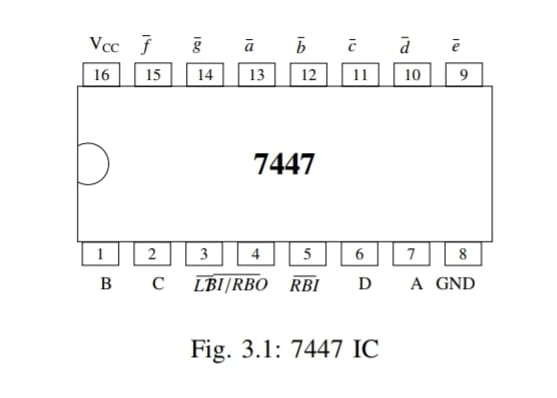
\includegraphics[width=\textwidth]{figs/7447.jpeg} 
    \end{minipage}
    \hfill
    \begin{minipage}{0.48\textwidth}
        \centering
        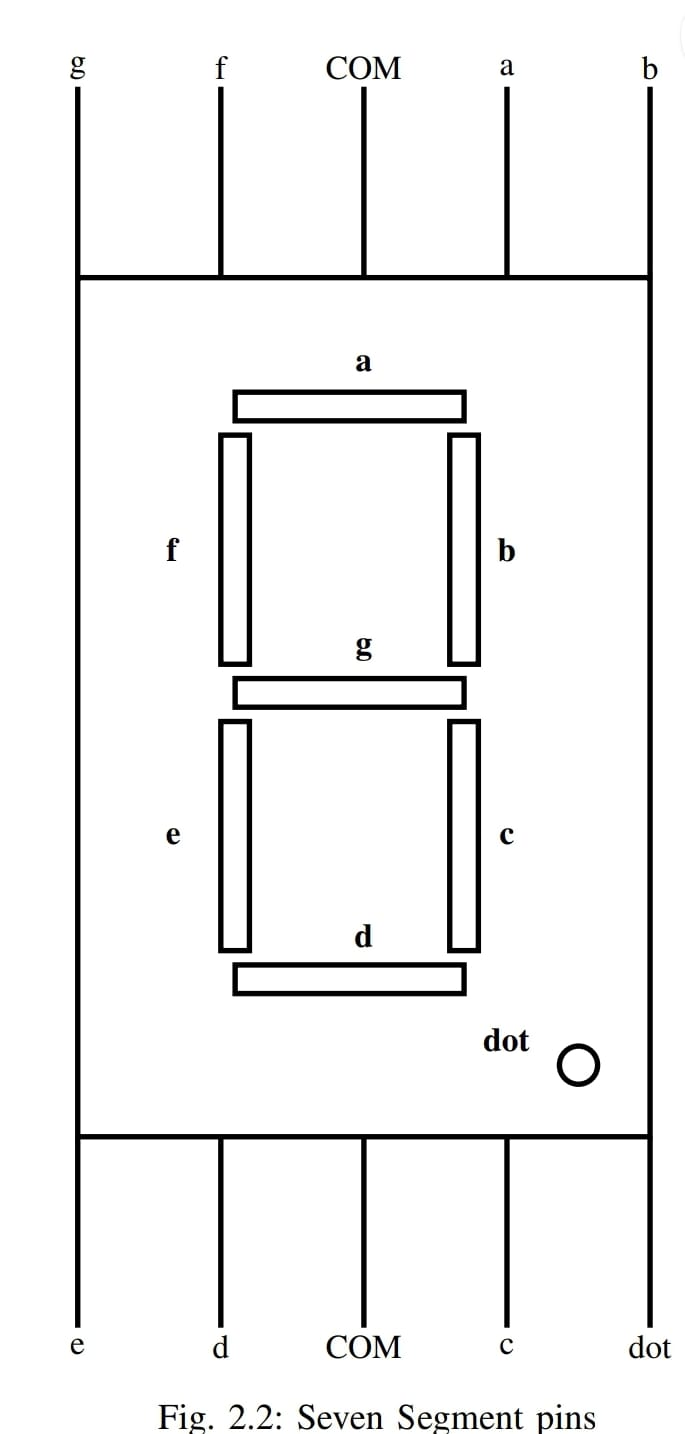
\includegraphics[width=\textwidth]{figs/seven_segment.jpeg}
    \end{minipage}
\end{figure}
\newpage

5$v$ pin of Arduino is connected to $v_{cc}$ of 7447 while their grounds are connected to each other.\\
\\
The COM pins of the 7-seg displays are connected to $220 \Omega$ which are connected to analogue pins on the Arduino.\\
\\
There are also 4 push buttons which are connected to 6,7,8 and 9 pins in the Arduino . They have the following uses
\begin{itemize}
    \item The first is used to adjust the hours of the clock by incrementing till 23 and then reset to zero.
    \item The second is used the adjust the minutes by incrementing till 59 then reset to zero.
    \item The third switches the clock between showing the time and being used as a stopwatch.
    \item The fourth is used to stop time or the stop watch.
\end{itemize}
The following is the picture of the fully functioning circuit
\begin{figure}[h!] % Another figure
  \centering
  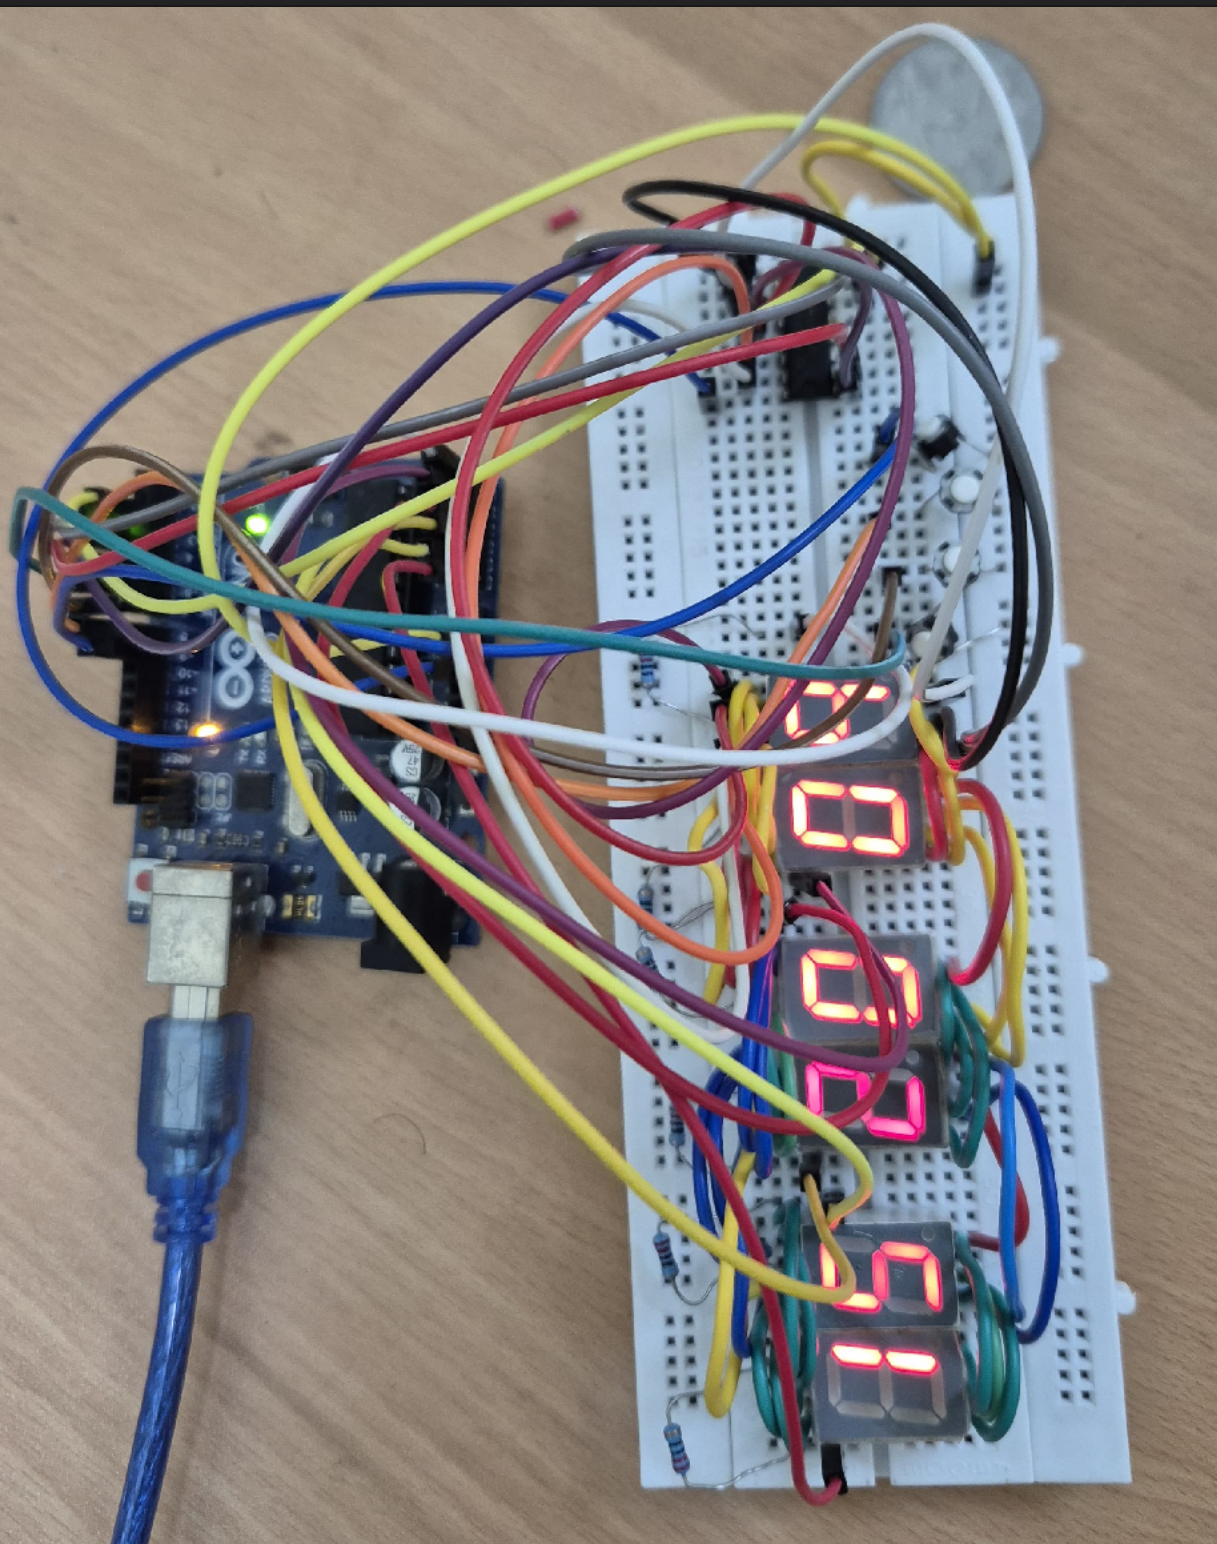
\includegraphics[width=0.6\textwidth]{figs/circuit.png}
\end{figure}

 \section{Code}
The following is the code implemented

\begin{lstlisting}{Language = c}
#define F_CPU 16000000UL
#include <avr/io.h>
#include <util/delay.h>
#include <avr/interrupt.h>

#define BCD_PORT PORTD
#define BCD_DDR DDRD
#define BCD_MASK 0b00111100  // PD2 to PD5

#define COMMON_PORT PORTC
#define COMMON_DDR DDRC

#define MODE_BUTTON PB0 // Switch between Clock, Timer, and Stopwatch
#define STOPWATCH_BUTTON PB1 // Start/Stop Stopwatch and Timer

volatile int seconds = 0, minutes = 0, hours = 15;
volatile int timer_seconds = 0, timer_minutes = 0, timer_hours = 0;
volatile int stopwatch_seconds = 0, stopwatch_minutes = 0, stopwatch_hours = 0;
volatile int mode = 0; // 0 = Clock, 1 = Timer, 2 = Stopwatch
volatile int stopwatch_running = 0; // 1 = Running, 0 = Stopped

void setup() {
    // Set BCD display pins (PD2-PD5) as output
    BCD_DDR |= BCD_MASK;
    BCD_PORT &= ~BCD_MASK;

    // Set digit selector pins (PORTC) as output
    COMMON_DDR = 0xFF;
    COMMON_PORT = 0x00;

    // Enable pull-up resistors for buttons
    PORTD |= (1 << PD6) | (1 << PD7);
    PORTB |= (1 << MODE_BUTTON) | (1 << STOPWATCH_BUTTON);

    // Timer1 Setup: CTC Mode, 1-second interval
    TCCR1B |= (1 << WGM12) | (1 << CS12) | (1 << CS10);
    OCR1A = 15625; // 1-second interrupt
    TIMSK1 |= (1 << OCIE1A);

    // Debug LED on PC7 (Bit 7 of PORTC) to check if ISR is running
    DDRC |= (1 << 7);  // Set PC7 as output
    PORTC &= ~(1 << 7); // Initially turn it off

    sei(); // Enable global interrupts
}

ISR(TIMER1_COMPA_vect) {
    PORTC ^= (1 << 7); // Toggle PC7 to check ISR is running

    // Clock Mode Updates
    if (mode == 0) {
        seconds++;
        if (seconds == 60) {
            seconds = 0;
            minutes++;
            if (minutes == 60) {
                minutes = 0;
                hours = (hours + 1) % 24;
            }
        }
    }

    // Timer Countdown (only when running)
    if (mode == 1 && stopwatch_running) {  
        if (timer_seconds > 0 || timer_minutes > 0 || timer_hours > 0) {
            if (timer_seconds == 0) {
                if (timer_minutes > 0) {
                    timer_minutes--;
                    timer_seconds = 59;
                } else if (timer_hours > 0) {
                    timer_hours--;
                    timer_minutes = 59;
                    timer_seconds = 59;
                }
            } else {
                timer_seconds--;
            }
        }
    }

    // Stopwatch Increment
    if (mode == 2 && stopwatch_running) {
        stopwatch_seconds++;
        if (stopwatch_seconds == 60) {
            stopwatch_seconds = 0;
            stopwatch_minutes++;
            if (stopwatch_minutes == 60) {
                stopwatch_minutes = 0;
                stopwatch_hours = (stopwatch_hours + 1) % 24;
            }
        }
    }
}

void displayTime();
void setBCD(int value);
void checkButtons();

int main() {
    setup();
    while (1) {
        checkButtons();
        displayTime();
    }
}

// Function to display time on a 6-digit 7-segment display
void displayTime() {
    int digits[6];

    if (mode == 0) { // Clock Mode
        digits[0] = hours / 10;
        digits[1] = hours % 10;
        digits[2] = minutes / 10;
        digits[3] = minutes % 10;
        digits[4] = seconds / 10;
        digits[5] = seconds % 10;
    } else if (mode == 1) { // Timer Mode
        digits[0] = timer_hours / 10;
        digits[1] = timer_hours % 10;
        digits[2] = timer_minutes / 10;
        digits[3] = timer_minutes % 10;
        digits[4] = timer_seconds / 10;
        digits[5] = timer_seconds % 10;
    } else { // Stopwatch Mode
        digits[0] = stopwatch_hours / 10;
        digits[1] = stopwatch_hours % 10;
        digits[2] = stopwatch_minutes / 10;
        digits[3] = stopwatch_minutes % 10;
        digits[4] = stopwatch_seconds / 10;
        digits[5] = stopwatch_seconds % 10;
    }

    // Multiplex 7-segment display
    for (int i = 0; i < 6; i++) {
        setBCD(digits[i]); // Send the BCD value first
        COMMON_PORT = (1 << i); // Enable the corresponding digit
        _delay_us(500); // Short delay for smooth display
    }
}

// Function to set BCD output for 7-segment display
void setBCD(int value) {
    BCD_PORT = (BCD_PORT & ~BCD_MASK) | ((value << 2) & BCD_MASK);
}

// Function to check button inputs and update mode/settings
void checkButtons() {
    if (!(PIND & (1 << PD6))) {
        _delay_ms(50);
        if (!(PIND & (1 << PD6))) {
            if (mode == 0) {
                hours = (hours + 1) % 24;
                seconds = 0;
            } else if (mode == 1) {
                timer_hours = (timer_hours + 1) % 24;
                seconds = 0;
            }
            while (!(PIND & (1 << PD6))); // Wait for release
        }
    }

    if (!(PIND & (1 << PD7))) {
        _delay_ms(50);
        if (!(PIND & (1 << PD7))) {
            if (mode == 0) {
                minutes = (minutes + 1) % 60;
                seconds = 0;
            } else if (mode == 1) {
                timer_minutes = (timer_minutes + 1) % 60;
                seconds = 0;
            }
            while (!(PIND & (1 << PD7))); // Wait for release
        }
    }

    if (!(PINB & (1 << MODE_BUTTON))) {
        _delay_ms(50);
        if (!(PINB & (1 << MODE_BUTTON))) {
            mode = (mode + 1) % 3; // Cycle through Clock, Timer, and Stopwatch
            while (!(PINB & (1 << MODE_BUTTON))); // Wait for release
        }
    }

    // Modified section: Stopwatch button controls both Timer and Stopwatch
    if (!(PINB & (1 << STOPWATCH_BUTTON))) {
        _delay_ms(50);
        if (!(PINB & (1 << STOPWATCH_BUTTON))) {
            if (mode == 2) {  // Toggle Stopwatch running
                stopwatch_running = !stopwatch_running;
            } else if (mode == 1) {  // Toggle Timer running
                stopwatch_running = !stopwatch_running;  // Reuse the same flag
            }
            while (!(PINB & (1 << STOPWATCH_BUTTON))) {
                _delay_ms(10);
            }
        }
    }
}
\end{lstlisting}

\section{Working of circuit based on the code}
\begin{itemize}
    \item \textbf{Clock Mode:} Displays and updates the current time in a 24-hour format.
    \item \textbf{Timer Mode:} Allows countdown from a set time.
    \item \textbf{Stopwatch Mode:} Tracks elapsed time when running.
\end{itemize}

A six-digit 7-segment display is used for output, and push buttons provide user interaction to switch modes and start/stop timing operations.

\section*{Pin Configuration and Display Control}

The system uses Binary-Coded Decimal (BCD) representation for displaying digits on the 7-segment display. The display is multiplexed, meaning only one digit is active at a time, and the microcontroller rapidly cycles through them to create a persistent visual effect.
\subsection*{BCD and Digit Selection}

\begin{lstlisting}
#define BCD_PORT PORTD
#define BCD_DDR DDRD
#define BCD_MASK 0b00111100  // PD2 to PD5

#define COMMON_PORT PORTC
#define COMMON_DDR DDRC
\end{lstlisting}

\begin{itemize}
    \item \textbf{BCD\_PORT (PORTD, PD2-PD5)} controls the segment encoding.
    \item \textbf{COMMON\_PORT (PORTC, PC0-PC5)} selects which digit to activate.
\end{itemize}

All these pins are set as outputs:

\begin{lstlisting}
BCD_DDR |= BCD_MASK;
COMMON_DDR = 0xFF;
\end{lstlisting}

\section*{Button Configuration}

Two push buttons are used for user input:

\begin{itemize}
    \item \textbf{Mode Button (PB0)} - Switches between Clock, Timer, and Stopwatch modes.
    \item \textbf{Start/Stop Button (PB1)} - Starts and stops the stopwatch or timer.
\end{itemize}

The buttons are connected with internal pull-up resistors to avoid floating states:

\begin{lstlisting}
PORTB |= (1 << MODE_BUTTON) | (1 << STOPWATCH_BUTTON);
\end{lstlisting}

\section*{Time Tracking Variables}
Three sets of time variables store hours, minutes, and seconds for each mode:

\begin{lstlisting}
volatile int seconds = 0, minutes = 0, hours = 15;
volatile int timer_seconds = 0, timer_minutes = 0, timer_hours = 0;
volatile int stopwatch_seconds = 0, stopwatch_minutes = 0, stopwatch_hours = 0;
\end{lstlisting}

\begin{itemize}
    \item \textbf{Clock mode} starts with an initial time (e.g., 15:00:00).
    \item \textbf{Timer mode} counts down when started.
    \item \textbf{Stopwatch mode} increments when running.
\end{itemize}

\section*{Interrupt-Driven Time Updates}

A hardware timer (Timer1) generates an interrupt every second to update time values.

\subsection*{Timer1 Configuration}

\begin{lstlisting}
TCCR1B |= (1 << WGM12) | (1 << CS12) | (1 << CS10);
OCR1A = 15625;
TIMSK1 |= (1 << OCIE1A);
\end{lstlisting}

\begin{itemize}
    \item Configures Timer1 in \textbf{CTC mode} (Clear Timer on Compare Match).
    \item Uses a prescaler of 1024 to achieve a 1-second interval.
    \item Triggers an interrupt when the timer reaches 15625 counts.
\end{itemize}

\subsection*{Interrupt Service Routine (ISR)}

Every second, the ISR updates the appropriate time variables based on the active mode.

\textbf{Clock Mode}

\begin{lstlisting}
if (mode == 0) {
    seconds++;
    if (seconds == 60) {
        seconds = 0;
        minutes++;
        if (minutes == 60) {
            minutes = 0;
            hours = (hours + 1) % 24;
        }
    }
}
\end{lstlisting}
\begin{itemize}
    \item Increments seconds.
    \item Rolls over to minutes and hours when necessary.
\end{itemize}

\textbf{Timer Mode}

\begin{lstlisting}
if (mode == 1 && stopwatch_running) {  
    if (timer_seconds == 0) {
        if (timer_minutes > 0) {
            timer_minutes--;
            timer_seconds = 59;
        } else if (timer_hours > 0) {
            timer_hours--;
            timer_minutes = 59;
            timer_seconds = 59;
        } } else {
        timer_seconds--;
    }
}
\end{lstlisting}

\textbf{Stopwatch Mode}

\begin{lstlisting}
if (mode == 2 && stopwatch_running) {
    stopwatch_seconds++;
    if (stopwatch_seconds == 60) {
        stopwatch_seconds = 0;
        stopwatch_minutes++;
        if (stopwatch_minutes == 60) {
            stopwatch_minutes = 0;
            stopwatch_hours = (stopwatch_hours + 1) % 24;
            }
    }
}
\end{lstlisting}

\begin{itemize}
    \item Increments time while running.
    \item Rolls over when needed.
\end{itemize}

\section*{7-Segment Display Multiplexing}
The function \texttt{displayTime()} handles time display:

\begin{lstlisting}
void displayTime() {
    int digits[6];

    if (mode == 0) { 
        digits[0] = hours / 10;
        digits[1] = hours % 10;
        digits[2] = minutes / 10;
        digits[3] = minutes % 10;
        digits[4] = seconds / 10;
        digits[5] = seconds % 10;
    }
    ...
    for (int i = 0; i < 6; i++) {
        setBCD(digits[i]); 
        COMMON_PORT = (1 << i); 
        _delay_us(500);
    }
}
\end{lstlisting}

\begin{itemize}
    \item Converts the current mode's time into six digits.
    \item Updates one digit at a time using BCD.
    \item Uses a short delay to ensure smooth display.
\end{itemize}

\section*{Button Handling}
The function \texttt{checkButtons()} reads button inputs and updates settings accordingly.

\begin{lstlisting}
if (!(PINB & (1 << MODE_BUTTON))) {
    _delay_ms(50);
    if (!(PINB & (1 << MODE_BUTTON))) {
        mode = (mode + 1) % 3; 
        while (!(PINB & (1 << MODE_BUTTON)));
    }
}
\end{lstlisting}

\begin{itemize}
    \item Checks if the mode button is pressed.
    \item Debounces input using a delay.
    \item Cycles through Clock, Timer, and Stopwatch.
\end{itemize}

The start/stop button toggles operation:

\begin{lstlisting}
if (!(PINB & (1 << STOPWATCH_BUTTON))) {
    _delay_ms(50);
    if (!(PINB & (1 << STOPWATCH_BUTTON))) {
        stopwatch_running = !stopwatch_running;
        while (!(PINB & (1 << STOPWATCH_BUTTON))) {
            _delay_ms(10);
        }
    }
}
\end{lstlisting}

\section{Results}
\begin{itemize}
    \item The clock is successfully able to display time.
    \item Stopwatch is also functioning correctly.
    \item Countdown timer also works perfectly.
    \item The push helps in easy controlling and adjustment of time in clock as well as the others     
\end{itemize}

\section{Conclusion}
This project implements a functional digital clock with help from Arduino. Although its simple, easy and functioning but there is still room for improvement.

\begin{thebibliography}{9}

\bibitem{ai_suggestions} AI Suggestions, Personal Recommendations.

\bibitem{hardware_guide} Hardware Connections Guide, Available from online sources.

\end{thebibliography}

\end{document}

